\documentclass[twoside]{article}


\usepackage[sc]{mathpazo} % Use the Palatino font
\usepackage[T1]{fontenc} % Use 8-bit encoding that has 256 glyphs
\linespread{1.3} % Line spacing - Palatino needs more space between lines
\usepackage{microtype} % Slightly tweak font spacing for aesthetics

\usepackage[hmarginratio=1:1,top=32mm,columnsep=20pt]{geometry} % Document margins
\usepackage{multicol} % Used for the two-column layout of the document
\usepackage[hang, small,labelfont=bf,up,textfont=it,up]{caption} % Custom captions under/above floats in tables or figures
\usepackage{booktabs} % Horizontal rules in tables
\usepackage{float} % Required for tables and figures in the multi-column environment - they need to be placed in specific locations with the [H] (e.g. \begin{table}[H])
\usepackage{hyperref} % For hyperlinks in the PDF

\usepackage{lettrine} % The lettrine is the first enlarged letter at the beginning of the text
\usepackage{paralist} % Used for the compactitem environment which makes bullet points with less space between them

\usepackage{titlesec} % Allows customization of titles
\renewcommand\thesection{\Roman{section}} % Roman numerals for the sections
\renewcommand\thesubsection{\Roman{subsection}} % Roman numerals for subsections
\titleformat{\section}[block]{\large\scshape\centering}{\thesection.}{1em}{} % Change the look of the section titles
\titleformat{\subsection}[block]{\large}{\thesubsection.}{1em}{} % Change the look of the section titles

\usepackage{fancyhdr} % Headers and footers
\pagestyle{fancy} % All pages have headers and footers
\fancyhead{} % Blank out the default header
\fancyfoot{} % Blank out the default footer
\fancyhead[C]{USC EE511-PROJECT4} % Custom header text
\fancyfoot[RO,LE]{\thepage} % Custom footer text



\usepackage{multicol}
\usepackage{listings}
\usepackage{graphicx}
\usepackage{caption}
\usepackage{subcaption}
\usepackage{hyperref}
\usepackage{color}
\usepackage{float}
\usepackage{mathtools}
\usepackage{amssymb}
\usepackage{wrapfig}


\lstset{ %
language=Matlab,                % choose the language of the code
basicstyle=\footnotesize,       % the size of the fonts that are used for the code
numbers=left,                   % where to put the line-numbers
numberstyle=\footnotesize,      % the size of the fonts that are used for the line-numbers
stepnumber=1,                   % the step between two line-numbers. If it is 1 each line will be numbered
numbersep=5pt,                  % how far the line-numbers are from the code
backgroundcolor=\color{white},  % choose the background color. You must add \usepackage{color}
showspaces=false,               % show spaces adding particular underscores
showstringspaces=false,         % underline spaces within strings
showtabs=false,                 % show tabs within strings adding particular underscores
frame=single,           % adds a frame around the code
tabsize=2,          % sets default tabsize to 2 spaces
captionpos=b,           % sets the caption-position to bottom
breaklines=true,        % sets automatic line breaking
breakatwhitespace=false,    % sets if automatic breaks should only happen at whitespace
escapeinside={\%*}{*)}          % if you want to add a comment within your code
}
%----------------------------------------------------------------------------------------
%	TITLE SECTION
%----------------------------------------------------------------------------------------

\title{\vspace{-15mm}\fontsize{24pt}{10pt}\selectfont\textbf{Project \#4 - Integrals and Intervals }} % Article title

\author{
\large
\textsc{Li Yicheng}\thanks{\href{https://github.com/IAMLYCHEE/EE501-PROJ4}{github link: https://github.com/IAMLYCHEE/EE501-PROJ4} }\\[2mm] % Your name
\normalsize USCID:7827077047\\
\normalsize email: l.y.c.liyicheng@gmail.com \\ % Your institution
\normalsize USC Viterbi of Engineering
\vspace{-5mm}
}

\date{}

%----------------------------------------------------------------------------------------

\begin{document}

\maketitle % Insert title

\thispagestyle{fancy} % All pages have headers and footers
\section{Computing Integrals and monte carlo simulation}
\subsection{\normalsize{Requirement}}
\noindent \textbf {Compute the following integrals}\\
\noindent \textbf {a:}$\int_{-2}^{2}\mathrm{e}^{x+x^2}\mathrm{d}x$
~~~~\textbf {b:}$\int_{-\infty}^\infty\mathrm{e}^{-x^2}\mathrm{d}x$
~~~~ \textbf {c:}$\int_0^1\int_0^1\mathrm{e}^{-(x+y)^2}\mathrm{d}y\mathrm{d}x$\\
\subsection{\normalsize{Experiment}}
\noindent \textbf {a: Monte Carlo Simulation}\\
The basic idea is $\int_0^1g(x)\mathrm{d}x = E(g(u))$ where \textbf{u} is samples draw from the standard uniform distribution. Actually it is easy to qualitativly prove this. For instance we have n samples $u_i$ draw from [0,1], then we divide the [0,1] into n pieces and assign width $1/n$ to each sample $u_i$, each sample has a height g($u_i$), and it has a corresponding area $\frac{1}{n}g(u_i)$. And we add all the areas together to simulate the value of the integral, it would be $\displaystyle\sum_{1}^{n}\frac{1}{n}g(u_i)$ and this is $E(g(u))$. The simulation can be accurate if lots of samples are drawn from the standard uniform distribution.To put this simulation method into application, the following three situations are discussed.\\
\noindent \textbf {*1} if we would like to integral $f(x)$, x range from a to b. We should first translate the range [a,b] to [0,1]. This is easy to be implemented by let $y = \frac{x-a}{b-a}$. In this case. Then compute the new $\mathrm{d}x$, at last we can derive the final formular: $\int_a^b g(x) \mathrm{d}x = (b-a)\int_0^1g((b-a)y + a)\mathrm{d}y$\\
\noindent \textbf {*2} if we would like to integral $f(x)$, x has an infinite range, say x from a(a>0) to $\infty$, we use the same idea in *1, we translate the range $x \in [a,\infty]$ to $y \in [0,1]$, this can be done by letting $y = \frac{1}{1+x-a}$, continue doing calculation we can finally get $\int_a^\infty g(x)\mathrm{d}x = \int_0^1 g(\frac{1}{y}+a-1)\frac{1}{y^2}\mathrm{d}y$\\
\noindent \textbf {*3} when it comes to the multiple integrals in the form like\\ $\int_{a_1}^{b_1}\int_{a_2}^{b_2}\cdots\int_{a_{n-1}}^{b_{n-1}}\int_{a_n}^{b_n}g(x_1,x_2,x_3\cdots x_n)\mathrm{d}x_1\mathrm{d}x_2\cdots\mathrm{d}x_n$. \\It is also easy to derive the simulation by translate each range to the [0,1], $x_n \rightarrow u_n, u_n \sim u[0,1]$ compute the $x_n = T(u_n)$, Therefore: $\int_{a_1}^{b_1}\int_{a_2}^{b_2}\cdots\int_{a_{n-1}}^{b_{n-1}}\int_{a_n}^{b_n}g(x_1,x_2,x_3\cdots x_n)\mathrm{d}x_1\mathrm{d}x_2\cdots\mathrm{d}x_n \\ = \int_0^1\int_0^1\cdots\int_0^1g(T_1(u_1),T_2(u_2)\cdots T_n(u_n))dT_1(u_1)dT_2(u_2)\cdots dT_n(u_n)$\\

\noindent \textbf {b.Implementation}\\
\noindent \textbf {*1}  Compute $\int_{-2}^{2}\mathrm{e}^{x+x^2}\mathrm{d}x$\\
\underline{filename}:  integral\_fi.m\\
\begin{lstlisting}
function result = integral_fi(a,b,eval_budget)
%b is the upper bound of the integral
%a is the lower bound of the integral
%eval_budget determines the amount of samples generated to evaluate
unif_samples = rand(eval_budget,1);
x = (b - a) * unif_samples + a; %y -> x
g_x = exp(x.^2 + x); %compute g(x)
result = (b - a).*mean(g_x);
\end{lstlisting}
\noindent \textbf {*2}  Compute $\int_{-\infty}^\infty\mathrm{e}^{-x^2}\mathrm{d}x$\\
\underline{filename}: integral\_inf.m\\
\begin{lstlisting}
function result = integral_inf(a,eval_budget)
%result = integral_inf(a,eval_budget)
%a : the input lower bound , a >= 0 
%eval_budget: the amount of samples to get the result 

y = rand(eval_budget,1)+1e-10; %y>0
x = y.^(-1) - (1 - a); %translate the range
%since this is an even symmetry function we only need to calculate half of the integral
result = 2*mean( exp(- x.^2) ./ (y.^2) ); 
\end{lstlisting} 
\noindent \textbf {*3}  Compute $\int_0^1\int_0^1\mathrm{e}^{-(x+y)^2}\mathrm{d}y\mathrm{d}x$\\
\underline{filename}: multi\_integ.m\\
\begin{lstlisting}
function result = multi_integ(eval_budget)
%result = multi_integ(va_amount, eval_budget)
%this is multiintegral with bound 0 to 1
%eval_budget: the amount of samples to draw
u = rand(eval_budget,2);
result = mean( exp( -1 * (u(:,1) + u(:,2)).^2));
\end{lstlisting}

\subsection{\normalsize{Result \& Analysis}}
\noindent \textbf {*1} \\
\noindent \textbf {query: result = integral\_fi(-2,2,10000) \\}
\noindent \textbf {result = 92.9909\\}
\noindent \textbf {theoretical result:\\
$result = -\dfrac{\mathrm{e}^{-\frac{1}{4}}\sqrt{{\pi}}\mathrm{i}\left(\operatorname{erf}\left(\frac{5\mathrm{i}}{2}\right)+\operatorname{erf}\left(\frac{3\mathrm{i}}{2}\right)\right)}{2}=93.16275329244197$}\\[10pt]



\noindent \textbf {*2}\\
\noindent \textbf {query: result = integral\_inf(0,15000)\\}
\noindent \textbf {result = 1.7801\\}
\noindent \textbf {theoretical result: \\
$result = \sqrt{{\pi}}= 1.772453850905516$}\\[10pt]

\noindent \textbf {*3}\\
\noindent \textbf {query: result = multi\_integ(15000)\\}
\noindent \textbf {result = 0.4111\\}
\noindent \textbf {theoretical result:\\ $result = \frac{1}{2 e^{4}} \left(- 2 e^{3} + 1 + 2 \sqrt{\pi} \left(- e^{4} \operatorname{erf}{\left (1 \right )} + e^{4} \operatorname{erf}{\left (2 \right )}\right) + e^{4}\right)\approx 0.411792894172914$}\\

\noindent \textbf {Performance Analysis\\}
Take the first integral for example, a bunch of different sample amount were input to test the accuracy.\\
\begin{multicols}{2}
\begin{figure}[H]
   \centering
   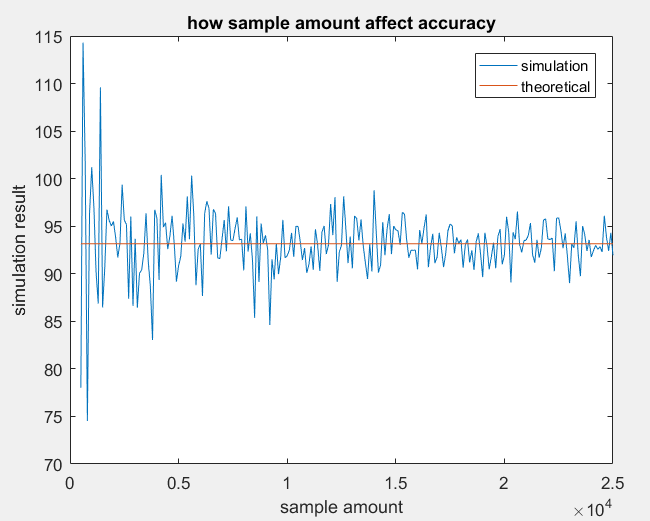
\includegraphics[width = 0.5\textwidth]{../data/accuracy1.png}  
   \caption{accuracy test}
\end{figure}
The sample amount vary from 500 to 25000, when the amount is small, large oscillation occurs and we may get 71.2339 as a simulation result which has a 21\% difference to the theoretical value. When the sample amount get larger, it become more and more stable to derive values fit to the theoretical value.Therefore, when use such simulation method, the sample amount should not be too small.\\
\end{multicols}

\newpage
\section{empirical distribution}
\subsection{\normalsize{Requirement}}
We have a random variable which is defined as $X= Z_1^2 +Z_2^2 +Z_3^2 +Z_4^2 $, and $Z$ conforms to the standard normal distribution. How to derive a distribution function of X by having 10 samples? Using the Empirical distribution to simulate the cdf of x and compare it to the theoretical cdf.\\

\subsection{\normalsize{Experiment}}
\noindent \textbf {Theory}\\
The idea of empirical distribution simulation is qualitatively easy to understand. We can first define x in some range. For instance, we let $x \in [0,15], x = nT, T = 0.01$. So we first choose $x = 0$, and find how many samples $\in (-\infty,0)$, then choose $x = 0.01$, find how many samples  $\in (-\infty,0.01)$, continue doing so until $x=15$. This form the empirical distribution.\\
\noindent \textbf {Algorithm}\\
\noindent \textbf {*1} Derive several samples.\\
\noindent \textbf {*2} Define the x range of the cdf.\\
\noindent \textbf {*3} Iterate x in the defined range and find the number of samples in the range.\\[10pt]
\noindent \textbf {Implementation}\\
\underline{filename}: generateF10x.m
\begin{lstlisting}
function Fn = generateF10x(sample,lb,ub,isplot)
%Fn = generateF10x(sample,lb,ub,isplot)
%generate the empirical distribution
%sample: the amount of samle 
%lb: the lower bound of x
%ub: the upper bound of x
%isplot: whether plot or not
X = zeros(sample, 1);
for i = 1 : sample 
    X(i) = sum( randn(4,1) .^2 );
end

k = length(lb: 0.05 : ub);
Fn = zeros(k , 1);
k = 1;
for x = lb : 0.05 : ub
    accsum = 0;
    for i = 1 : sample
        if X(i) < x
            accsum = accsum + 1;
        end
    end
    Fn(k) = accsum/sample;
    k = k + 1; 
end
if isplot
    plot((lb:0.05:ub),Fn);
    hold on 
    x = lb : 0.05 : ub;
    F_the = chi2cdf(x , 4);
    plot( x , F_the)
    hold off 
    xlabel('x')
    ylabel('probability')
    title('empirical distribution')
    legend('Empirical Simulation','theoretical')
end
\end{lstlisting}
To further compute $||F_{10}^*(x)-F(x)||_\infty$ and the $25^{th},50^{th},90^{th}$ percentiles using empirical distribution and compare it to the theoretical value with the following script.\\
\underline{filename}:solution2.m\\
\begin{lstlisting}
%generate the theoretical chi-square distribution cdf
x = 0 : 0.05 : 10;
F_the = chi2cdf(x , 4);
F_the = F_the';
%generate simulation with 10 samples
Fn = generateF10x(10,0,10,true);
%compute differences
diff = abs( Fn - F_the );
maxDiff = max(diff);

xSize = length(x);
e25 = Fn(round(xSize*0.25));
e50 = Fn(round(xSize*0.50));
e90 = Fn(round(xSize*0.90));
the25 = F_the(round(xSize*0.25));
the50 = F_the(round(xSize*0.50));
the90 = F_the(round(xSize*0.90));
\end{lstlisting}

\subsection{\normalsize{Result \& Analysis}}
\newpage
\begin{multicols}{2}
\begin{figure}[H]
   \centering
   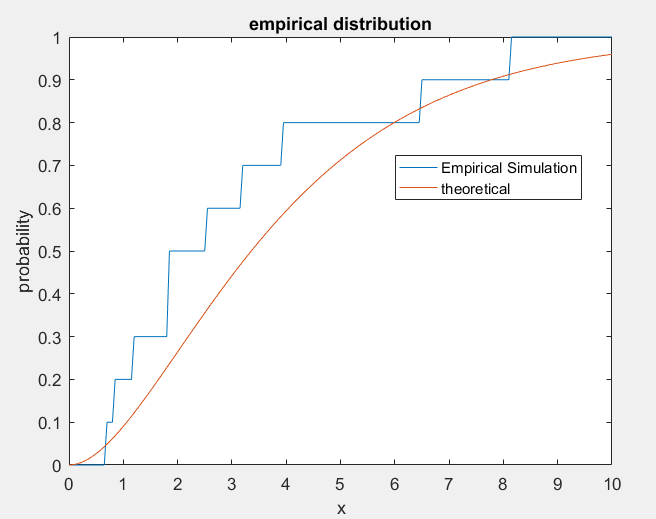
\includegraphics[width = 0.4\textwidth]{../data/solution2.png}  
   \caption{Empirical Distribution}
\end{figure}
\noindent \textbf {Result:\\[15pt]}
\begin{tabular}{|| c | c | c ||}
 \hline \hline
 $n^{th} percentile$ & empirical  & theoretical \\ \hline \hline
25 & 0.2000 & 0.3464 \\ \hline
50 & 0.7000 & 0.7127\\ \hline
90 & 0.9000 & 0.9389\\ \hline
\end{tabular}
maximum difference = 0.2422.
\end{multicols}
The max difference between empirical distribution and theoretical distribution is 0.2422. This seems to be a large difference when it comes to probability. However, when $Pr(X<=x)$ is near 1, the empirical distribution approaches theoretical distribution. That is, for the $x^th$ percentiles, the more x approaches 1, the difference between $F_{10}^*(x) \ and \ F(x)$. \\[15pt]
If the sample amount is 100, we get another result:\\
\begin{multicols}{2}
\begin{figure}[H]
   \centering
   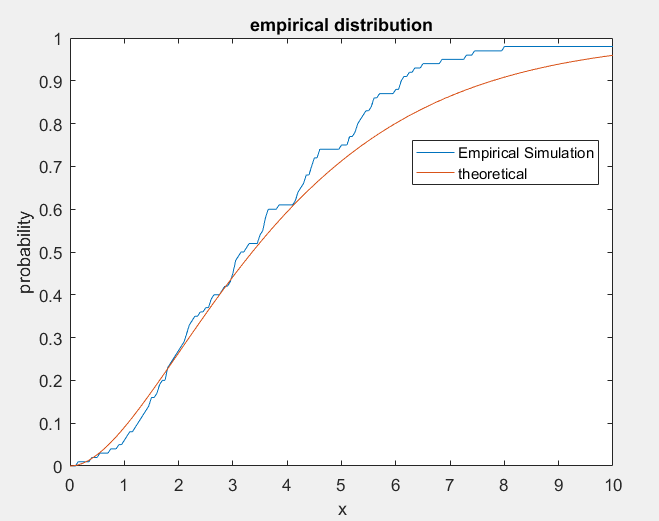
\includegraphics[width = 0.4\textwidth]{../data/sample100.png}  
   \caption{Empirical Distribution}
\end{figure}
\noindent \textbf {Result:\\[15pt]}
\begin{tabular}{|| c | c | c ||}
 \hline \hline
 $n^{th} percentile$ & empirical  & theoretical \\ \hline \hline
25 & 0.3500 & 0.3464 \\ \hline
50 & 0.7600 & 0.7127\\ \hline
90 & 0.9500 & 0.9389\\ \hline
\end{tabular}
maximum difference = 0.0663.
\end{multicols}

\section{confidence interval}
\subsection{\normalsize{Requirement}}
We have a data file recording a geyser's eruption time and waiting time. The data has the population size 272. However, we estimate the waiting time and erruption time using only the first 15 samples. Derive the confidence interval using the 15 data samples, and compare it to the confidence interval of the whole population.\\
\subsection{\normalsize{Experiment}}
\noindent \textbf {a:Confidence Interval}\\
The statistical confidence interval uses the Z-distribution and conforms $(m-\frac{s}{\sqrt{n}}z_{\alpha/2},m+\frac{s}{\sqrt{n}}z_{\alpha/2})$ for a $100(1-\alpha)\%$ confidence interval. Here m is the observed value of sample mean. and s be the standard deviation.\\
Generate two functions, one is to compute the confidence interval, the other to compute the bootstrap confidence interval. \\
\noindent \textbf {b.Implementation}\\
\underline{filename}: computeCI.m\\
\begin{lstlisting}
function [mu,var] = computeCI(data,sampleAmount)
%compute the comfidence interval for the mean and standard deviation
%data: the input data
%sampleAmount: the amount of sample from the data
dataSample = data(1:sampleAmount);
pd = fitdist(dataSample,'Normal');
CI = paramci(pd);
mu = CI(:,1);
var = CI(:,2);
\end{lstlisting}
\underline{filename}: computeBootstrapCI.m\\
\begin{lstlisting}
function [mu,var]=computeBootstrapCI(data,sampleAmount)
%compute the bootstrap confidence interval for the mean and standard deviation
%data: the input data
%sampleAmount: the amount of sample from the data
data = data(1:sampleAmount);
dataMean = mean(data);
dataVars = abs(data - dataMean);
data=sort(data);
dataVars = sort(dataVars);
mu = [data(ceil(sampleAmount * 0.025)),data(ceil(sampleAmount*0.975))];
var = [dataVars(ceil(sampleAmount * 0.025)),dataVars(ceil(sampleAmount*0.975))];   
\end{lstlisting}
\underline{query script: }\\
\begin{lstlisting}
data = load('duration.mat');
duration = data.duration;
data = load('waiting.mat');
waiting = data.waiting;
[durationMu_15,durationVar_15] = computeCI(duration,15);
[durationMu_po,durationVar_po] = computeCI(duration,length(duration));
[waitingMu_15,waitingVar_15] = computeCI(waiting,15);
[waitingMu_po,waitingVar_po] = computeCI(waiting,length(waiting));
[durationMu_15_bootstrap,durationVar_15_bootstrap] = computeBootstrapCI(duration,15);
[durationMu_po_bootstrap,durationVar_po_bootstrap] = computeBootstrapCI(duration,length(duration));
[waitingMu_15_bootstrap,waitingVar_15_bootstrap] = computeBootstrapCI(waiting,15);
[waitingMu_po_bootstrap,waitingVar_po_bootstrap] = computeBootstrapCI(waiting,length(waiting));
\end{lstlisting}
\subsection{\normalsize{Result \& Analysis}}
\begin{multicols}{2}
\begin{figure}[H]
   \centering
   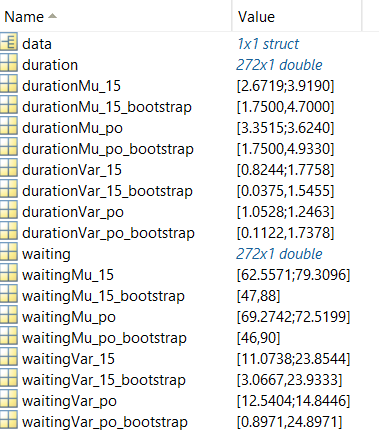
\includegraphics[width = 0.5\textwidth]{../data/data.png}  
\end{figure}
The left shows the confidence interval of the mean and the deviation.If we qualitatively plot these confidence intervals, we would have the following figure: \\
\begin{figure}[H]
   \centering
   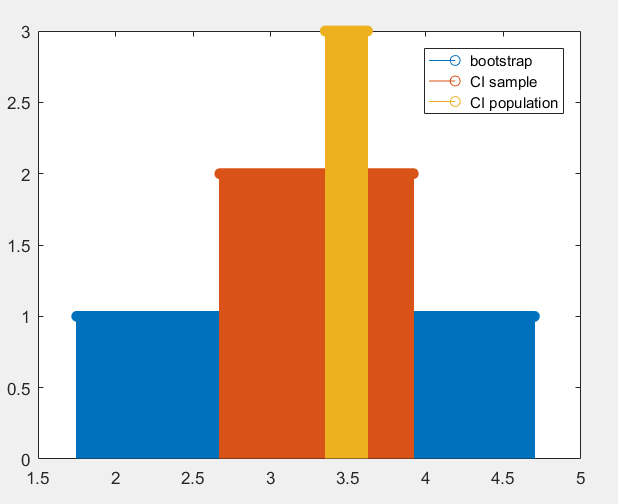
\includegraphics[width = 0.5\textwidth]{../data/analyse6.png}  
\end{figure}
\end{multicols}
From the figure, we can see that there exist a shift betwwen the 15 samples and the whole population, this means given the first 15 samples the estimation can be not accurate enough.  The statistic confidence interval tries to gather the two sides' information to the mid using the normal distribution assumption and thus performs better than the bootstrap confidence interval result.
\end{document}